%
% Demba Ba - NSF Biosketch
%
\pdfminorversion=4
\documentclass[12pt]{article}

\makeatletter
\let\saved@bibitem\@bibitem % < -- save to prevent problems due to the command getting redefined...
\makeatother

\usepackage{graphicx}
\usepackage{etaremune}
\usepackage[usenames,dvipsnames]{xcolor}
\usepackage{bibentry}
\PassOptionsToPackage{hyphens}{url}\usepackage[dvips]{hyperref}
\usepackage{geometry}
\usepackage[yyyymmdd,hhmmss]{datetime}
\urlstyle{same}

\usepackage{amsmath}
\usepackage{draftwatermark}
\SetWatermarkText{Confidential}
%\SetWatermarkScale{5}

% Fonts
\ifdefined\ispdf
    \usepackage[urw-garamond]{mathdesign}
    \usepackage[T1]{fontenc}
\else
    \usepackage[T1]{fontenc}
\fi

\def\HCode#1{}

% Set your name here
\def\name{Demba Ba}

% The following metadata will show up in the PDF properties
\hypersetup{
  colorlinks = true,
  urlcolor = gray,
  pdfauthor = {\name},
  pdfkeywords = {signal processing, computational neuroscience, scientific computing},
  pdftitle = {\name: Novel Brain-Machine Interfaces Using Deep Sparse Signal Representations and Multiscale Autoencoders},
  pdfsubject = {Deep Sparse Signal Representations},
  pdfpagemode = UseNone
}


\geometry{
  body={6.5in, 9.0in},
  left=1.0in,
  right=1.0in,
  top=1.0in
}

% Customize page headers
%%\pagestyle{myheadings}
%\markright{\name, Harvard University}
%\thispagestyle{empty}

% Custom section fonts
\usepackage{sectsty}
\sectionfont{\rmfamily\mdseries\Large}
\subsectionfont{\rmfamily\mdseries\itshape\large}

% Other possible font commands include:
% \ttfamily for teletype,
% \sffamily for sans serif,
% \bfseries for bold,
% \scshape for small caps,
% \normalsize, \large, \Large, \LARGE sizes.

% Don't indent paragraphs.
\setlength\parindent{0em}

% Make lists without bullets and compact spacing
\renewenvironment{itemize}{
  \begin{list}{}{
    %\setlength{\leftmargin}{1.5em}
    \setlength{\itemsep}{0.25em}
    \setlength{\parskip}{0pt}
    \setlength{\parsep}{0.25em}
  }
}{
  \end{list}
}

%To highlight my own name in the bibliography
\def\FormatName#1{%
    \def\myname{Demba Ba}%
    \edef\name{#1}%
    \ifx\name\myname
      \textbf{#1}%
    \else
      #1%
    \fi
}

\begin{document}
\sloppy

\begingroup
\makeatletter
\let\@bibitem\saved@bibitem % <-- restore the original command immediately before use
\nobibliography{include/all}
\endgroup

% Place name at left
%\HCode{<div style="margin: 0 auto; overflow: hidden; width: 960px">} %row
\HCode{<div class="fluid-container"}

%\HCode{<div style="display: inline; float: left; margin: 0 10px; overflow: hidden; width: 820px">} %column
\HCode{<div class="row">}
\HCode{<div class="col-md-12">}
\HCode{<h1>}
{\huge \name}
\HCode{</h1>}
\HCode{</div>} %column
\HCode{</div>} %row

\bigskip

\HCode{<div class="row">}
\HCode{<div class="col-md-4">}
\begin{minipage}[t]{0.5\textwidth}
  Assistant Professor of Electrical Engineering \\
  and Bioengineering \\
  Harvard University \\
  School of Engineering and Applied Sciences \\
  Maxwell Dworkin \\
  33 Oxford st
  Cambridge, MA 02138 \\
\end{minipage}
\HCode{</div>} %end column
\HCode{<div class="col-md-8">}
\begin{minipage}[t]{0.5\textwidth}
  Phone: (617) 496-1228 \\
  %Fax: (301) 332-5264 \\
  %Office: MD 143 \\
  Email: \href{mailto:demba@seas.harvard.edu}{demba@seas.harvard.edu} \\
  Homepage: \href{http://demba-ba.org/}{http://demba-ba.org/} \\
  Group page: \href{http://crisp.seas.harvard.edu}{http://crisp.seas.harvard.edu/}
\end{minipage}
\HCode{</div>} %end column
\HCode{</div>} %end row

\begin{center} {\large \textbf{Novel Brain-Machine Interfaces Using Deep Sparse Signal Representations and Multiscale Autoencoders}}%Theory, Algorithms, and Applications to Multiscale Fusion}}
\end{center}


\HCode{<div class="row">}
\HCode{<div class="col-md-12">}
%\section*{Professional Preparation}
%
%%\begin{itemize}
%%    \item Ph.D./M.S. EECS, Massachusetts Institute of Technology, 2011/2016.
%%    %\item M.S. EECS, Massachusetts Institute of Technology, 2006.
%%    \item B.S. Electrical Engineering, University of Maryland, College Park, 2004.
%%\end{itemize}
%
%%\hspace{-0.075in}
%\begin{tabular}{llll}
%University of Maryland & College Park, MD & Electrical Engineering & B.S., 2004 \\
%Massachusetts Institute of Technology & Cambridge, MA & Electrical Engineering & M.S., 2006 \\
% &  & and Computer Science & \\
%Massachusetts Institute of Technology & Cambridge, MA & Electrical Engineering & Ph.D., 2011 \\
% &  & and Computer Science & \\
%Massachusetts Institute of Technology & Cambridge, MA & Computational & 2011--2015 \\
% &  & and Neuroscience & \\
%
%\end{tabular}

\section*{Vision}

%Over the past decade, human interaction with a variety of sensors that monitor and/or alter the activity of the autonomic (e.g. wearable bands~\cite{savage2015mobile}) and central nervous system~\cite{sejnowski2014putting} has grown exponentially. One salient feature of these sensor data is their heterogeneity, i.e. the presence of different temporal and spatial scales, as well as categories. At present, there lack principled approaches that can fuse heterogeneous sources of data acquired at multiple temporal and spatial scales to identify common underlying latent multiscale states. More specifically, there is a need for a framework that can learn low-dimensional (e.g. sparse) latent representations of a system observed through high-dimensional multiscale observations, to obtain a provably adequate characterization of said system (e.g. heart or brain region/system), and then be used to design artificial intelligence (AI) algorithms to control desired states of the system.

\textbf{My goal is to develop artificial systems/human-machine interfaces that can seamlessly integrate data at multiple spatial and temporal scales to make intelligent decisions.} %The primary motivation for this is my work in computational neuroscience and my interest in developing next generation Brain-Machine Interfaces (BMIs) that can utilize data at multiple spatial and temporal scales.  
The classical example of a human-machine interface is a prosthetic limb. The artificial intelligence (AI) in a such devices relies on (a) models of limb kinematics, and (b) sensors to acquire muscle activity from the limb. Surface electromyography (EMG) is a non-invasive way to acquire such data. In certain cases, one must resort to invasive sensing methods such as depth EMG electrodes that are able to sense muscle activity at better temporal resolution and than surface EMG electrodes, but typically poorer spatial resolution. How does one optimally fuse these multiscale data to develop a more accurate AI system/Brain/Body-machine interface (BMI)? \textbf{In collaboration with colleagues at the Harvard Wyss Institute, I would like to build a prosthetic limb that uses a new framework I have developed, termed \emph{Deep Sparse Representations of Signals} (DSRS), and novel multiscale deep network architectures to significantly improve performance.} %The above is but one example of where the fusion of multiscale data is important in developing AI systems that can interact with the brain--so-called brain-machine interfaces (BMIs)--or the human body (wearables, e.g. fitbit).
\\
\\
As prior work, the SMuRF~\cite{smurf2017} model developed in my group (currently in press at \emph{Neural Computation}) is an example of a shallow multiscale representation. As I detail below, DSRS are motivated by the theory of filter banks in signal processing, and are related to deep neural networks. Figuring out the exact connections is a current exciting topic of research my group is pursuing. Interestingly, DSRS suggest alternatives to backpropagation for estimating deep neural network architectures (some details below). Moreover, they can provide some theoretical estimates for the number of training examples required to train such representations. Lastly, they provide a natural way to solve the multiscale fusion problem outlined above. Therefore, they can be naturally embedded in multiscale AI systems/BMI applications. 
\\
\\
Beyond neuroscience and BMIs, multiscale data fusion is an important problem in a number of other domains such as seismology, water resource management, cross-modal imaging of the earth, to only name a few. \textbf{This research will therefore impact any area where the fusion of multiscale data is important to build AI systems}.

%\subsection*{Motivation}
%
%Stochastic processes that exhibit dynamics at multiple temporal or spatial
%scales are pervasive in engineering and science. In health monitoring and neuroscience, there has been an increasing interest in taking a systems engineering approach to understanding and controlling the dynamics of the human body and the brain~\cite{kim2011epidermal2,liberman2013closed}. Indeed, over the past decade, human interaction with a variety of sensors that monitor and/or alter the activity of the autonomic (e.g. wearable bands~\cite{savage2015mobile}) and central nervous system~\cite{sejnowski2014putting} has grown exponentially. One salient feature of these sensor data is their heterogeneity, i.e. the presence of different temporal and spatial scales, as well as categories. At present, there lack principled approaches that
%can fuse heterogeneous sources of data acquired at multiple temporal and spatial scales to identify
%common underlying latent multiscale states. More specifically, there is a need for a framework that can learn low-dimensional (e.g. sparse) latent representations of a system observed through high-dimensional multiscale observations, to obtain a provably adequate characterization of said system (e.g. heart or brain region/system), and then be used to design algorithms to control desired states of the system. I propose to develop a theoretical and algorithmic framework for estimation, inference and model comparison in \emph{Deep Sparse Representations of Signals}, with applications to the fusion of information from multiscale sources. 

\section*{Aims and Timeline of Proposed Research}

The aims of the research I propose consist of practical (e.g. implementations, research output), as well as theoretical and scientific ones.

\subsection*{Practical Aims and Timeline of Proposed Research}


The concrete aims and timeline of the proposed research are 
\begin{enumerate}

	\item To use DSRS to develop new, faster, and more scalable training algorithms for deep architectures (\textbf{Expected completion: June 2018}).
	
	\item To implement these new training algorithms using Keras and Tensorflow on the AWS platform, and to make these implementations available to the community. My students and I are be excited to familiarize ourselves with Apache MXNet and the Gluon interface on AWS, and to implement our algorithms on the platform (\textbf{Expected completion: December 2018}).
	
	\item To develop multiscale autoencoder architectures that can be trained with backpropagation, implement these using Keras and TensorFlow, as well as Apache MXNet and Gluon, and compare their performance to those built with DSSR (\textbf{Expected completion: June 2019}).	
	
	\item To use DSRS to fuse multiscale BMI data and assess improvements in BMI quality. In particular, in collaboration with Robotics colleagues at the Harvard Wyss Institute, I will develop a DSRS/multiscale-encoder powered prosthetic (\textbf{Expected completion: June 2020}).
	
	\item To release Python open-source software on github that will implement the algorithms for fusing multiscale data and their use in BMIs (\textbf{Expected completion: incrementally during course of project}).

\end{enumerate}

\subsection*{Theoretical and Scientific Aims}

The research proposed here will provide answers to novel theoretical and algorithm questions. I plan to apply the theory and algorithms to answer scientific questions in computational neuroscience and mulsticale AI system design for neuroscience applications.
\\
\\
\noindent \textbf{\underline{Theoretical and Algorithmic aims}}: The proposed framework raises important, unanswered, theoretical and algorithmic questions 

\begin{enumerate}
	\item What are the connections between neural networks and filter banks with sparsity constraints?  What are the sparse recovery limits (e.g. number of measurements) of training a deep sparse filter bank model?
	
	\item How to train a deep sparse filter bank using ``small'' data? This is a problem that is particularly important in neuroscience where the size of the training data can in no sense be considered ``big''?
	
	\item How to develop efficient optimization algorithms to estimate deep sparse signal representations? These will be convex optimization problems that will need to be parallelized in clever ways, e.g using new ADMM algorithms.	
	
\end{enumerate}

\noindent \textbf{\underline{Scientific Aims}}: \emph{Deep Sparse Representations of Signals} provide a framework for answering important questions about the brain and the nature of neural computation. Examples of such questions are
\begin{enumerate}
	%\item What is the nature of interaction between neural data at different spatial and temporal scales (e.g. neural spiking and LFP)? How to fuse, in a statistically-optimal sense, multiscale data?
	\item What are the atoms of neural computation? How to learn, using multiscale neural data, the ``filters'' or atoms the brain uses to encode information?
	
	\item In a given application, e.g. a prosthetic limb, what are the temporal scales that are important to guarantee a certain level of performance/accuracy?

\end{enumerate}

\section*{Budget and Personnel}

I am requesting funds to support $3$ graduate students and myself. The funds will be used to fund one graduate student, Diana (Yingzhuo) Zhang, currently in her second year, during her third and fourth years. Diana is the author first author on the SMuRF algorithm~\cite{smurf2017}. The funds will also be used to support two current first-year students during their second year, one female (Bahareh Tolooshams) and one male (Edward Novikov). The funds requested for the students will also contribute towards travel to conferences, as well as their participation in CS/EE professional societies. Together, these students combine an interdisciplinary background in computer science, electrical engineering and signal processing that will be crucial in the execution of this project. At present, the funds requested for myself will contribute towards travel to conferences and salary during summer months. Figure~\ref{fig:budget} provides details of this preliminary budget. 
\\
\\
I would also like to request $\$10,000$ of AWS credits for myself and $\$10,000$ of AWS credits for each of my students, for a total of $\$40,000$. We will use these credits for development and prototyping work on p2.xlarge current-generation GPU instances. 

\begin{figure}[!h]
  \begin{center}
    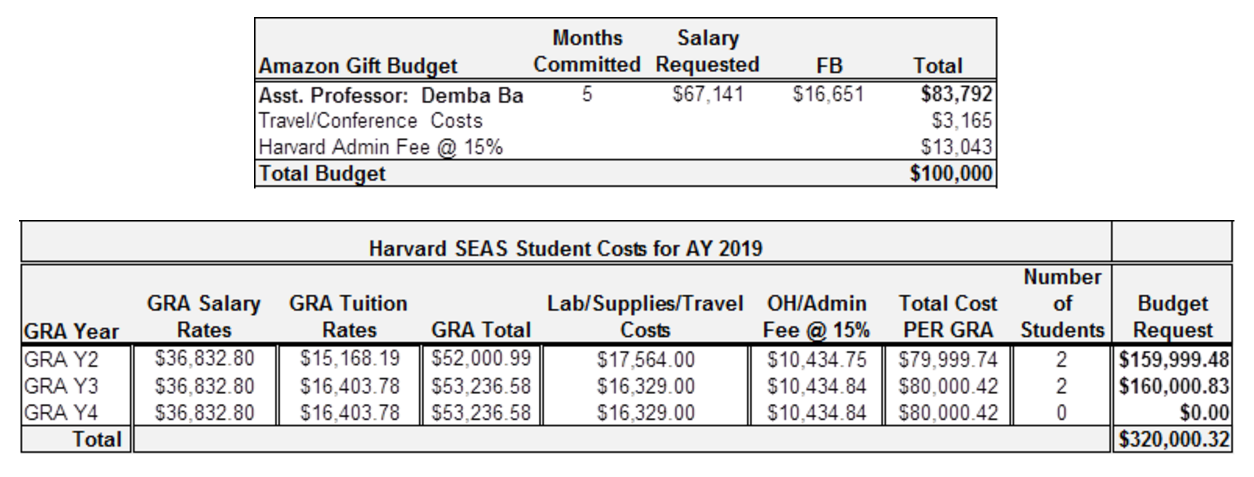
\includegraphics[scale=0.8]{AmznBudget.eps}
  \end{center}
  \vspace{-0.3in}
  \caption{Preliminary budget}
  \label{fig:budget}
\end{figure}

%I am asking for \$50,139 to fund one third-year Computer Science graduate student from September 1$^\text{st}$ 2016 to August 31$^\text{st}$ 2017. Of this amount, \$35,402 will cover the student's salary, and the remaining \$14,737 the cost of tuition. The said student has solid training in Statistics and numerical computing. This project will be a valuable learning opportunity to the student and will form a part of their dissertation.

\section*{Publication Venues}

I plan to submit the proposed work to the following conferences and journal publications

\begin{itemize}
	\item IEEE Statistical Signal Processing (SSP) workshop (\emph{Conference, June 10--June 13 2018})
	\item NIPS 2018 (Conference, \emph{December 3--December 8 2018})
	\item IEEE Transactions on Signal Processing (\emph{Journal, December 2018})
	\item ICML 2019 (\emph{Conference})
	\item Neural Compuation (\emph{Journal, December 2019})
	\item IEEE Transactions on Neural Systems and Rehabilitation Engineering (\emph{Journal, June 2020})
\end{itemize}



\section*{Deep Sparse Signal Representations: Theory, Algorithms and Applications}


\subsection*{Deep Sparse Signal Representations}

\emph{Deep Sparse Representations of Signals} are a generative model for multiscale stochastic processes that combines filter-bank theory~\cite{fliege1994multirate,strang1996wavelets,daubechies1992ten}, sparse recovery and compressed sensing~\cite{donoho2006compressed,candes2008introduction}, and state-space models~\cite{Ba:12,ba2013b}, to arrive at a signal processing/systems perspective and interpretation of deep neural networks. As detailed below, this new perspective provides several theoretical and algorithmic advantages over the classical approaches to deep neural networks~\cite{lecun2015deep}. Moreover, it provides a natural solution to the problem of fusing data from multiple spatial and temporal scales, an important problem in computational neuroscience (and numerous other scientific fields), high-resolution video/imaging and medical imaging.


\subsection*{Deep Sparse Filter Banks: a principled alternative to deep neural nets}

Deep architectures~\cite{lecun2015deep} for neural networks, and the accompanying learning algorithms,  have seen a resurgence over the past few years. One of the key appeals of deep learning has been its ability to yield predictive (e.g. class membership, cat or dog) hierarchical representations of nonlinear phenomena without the need for sophisticated a priori feature selection. The recent advances and success in a number of AI-related applications~\cite{bengio2009learning} are primarily a result of advances in computing and our ability to process massive amounts of data. One limitation of deep learning is the need for massive amounts of labelled data for learning. At present, there is significant interest in probabilistic generative models of deep networks~\cite{patel2015probabilistic} that do not require labelled data. %From a Bayesian perspective, generative models are appealing in small-data contexts as they allow one to balance prior and likelihood. From a Bayesian generative perspective, one reason why deep learning works is that access to massive amounts of data results in concentration of the posterior distribution  (data appears in likelihood term), so that the prior becomes less important. 
In classical signal processing and harmonic analysis, \emph{linear} multirate systems~\cite{fliege1994multirate} and filter banks~\cite{strang1996wavelets,daubechies1992ten} are the canonical framework for obtaining hierarchical representations of signals (analysis), and for generating signals from these representations (synthesis). I am developing a framework for studying deep generative hierarchical representations of signals based on \emph{nonlinear} filter banks. In linear filter banks, the filters in a given bank are specified as part of the synthesis step, allowing the \emph{generation} of signals. The \emph{Deep Sparse Filter Bank} framework shows that specifying an architecture for a neural network is in fact akin to specifying an analysis operator. The filters in the filter bank (synthesis) are related to the weights in a neural network, although there is not a one-to-one mapping between the two. Given the filters, the coefficients from the analysis step of the filter correspond to the hidden nodes in the network. Sparsity, and its interpretation as soft-thresholding in certain settings, provides the crucial nonlinearity that is one of the key components behind the success of deep architectures. The interpretation proposed here of deep architectures as nonlinear filter banks presents several advantages over current approaches

\begin{enumerate}
	\item \underline{Alleviating the computational burden in ``big''-data problems}: One current challenge in the training of deep networks is the need to store the data to be used for training on chip/on GPU. Relating deep architectures to compressed sensing and the theory of sparse recovery and high-dimensional statistics opens the door for ideas such as being able to estimate a deep network using random projections of the training data. This can lead to massive, theoretically-quantifiable, savings in terms of storage requirements, as well as practical algorithms.

	\item \underline{Learning deep filter banks from ``small'' data}: Generative models are all the more appealing in ``small''-data contexts as they allow one to balance the prior and likelihood. In experimental neuroscience, where the cost of training and acquiring data from animals (e.g. vision experiments with monkeys) can become prohibitive over time, being able to train deep networks is a challenge at the moment because of the limited amount of data that are available. The framework proposed here based on generative model and sparsity lends itself naturally to Bayesian inference and estimation, which allows the incorporation and quantification of the uncertainty in network-weight estimates that result from ``small'' data.
	
	\item \underline{A signal processing perspective}: Lastly, despite the rich theory of linear multirate systems and filter banks in signal processing and harmonic analysis, there lacks in the literature (beyond the work of Mallat for convolutional networks~\cite{bruna2013invariant}) a signal processing perspective to deep networks. Such a perspective would be a tremendous addition to the literature.
		
\end{enumerate}

%\section*{Current Funding}
%
%\section*{Pending Funding}

%\section*{Most Closely Related Publications}

%\subsection*{Published}
\ifdefined\ispdf
\begin{etaremune}
\else
\begin{enumerate}
\fi
	\item \bibentry{smurf2017}.
	\item \bibentry{zhang2017smurf}.
	\item \bibentry{schamberg2017modularized}.
	\item \bibentry{czanner15}.
    \item \bibentry{ba2013b}.
\ifdefined\ispdf
\end{etaremune}
\else
\end{enumerate}
\fi

%\subsection*{Accepted}

%\begin{enumerate}
%\end{enumerate}

%\subsection*{Submitted}
%\begin{enumerate}
%\end{enumerate}


%\subsection*{In preparation}

%\begin{enumerate}
	%\item \bibentry{mitchell2013}.
	%\item \bibentry{foster2013}.
	%\item \bibentry{york2013}.
%\end{enumerate}

%\subsection*{In Review}
%\begin{enumerate}
%\end{enumerate}



%\section*{Appointments}
%
%\begin{itemize}
%    \item Harvard University, \emph{Assistant Professor of Electrical and Bioengineering (July 2015--Present)}
%
%    \item MIT Neuroscience Statistics Research lab, \emph{RA/Post-doc fellow (Sep. 2007--Aug. 2014)}
%
%    \item Google -- \emph{Summer Intern (June 2010--September 2010)}
%
%    \item Microsoft Research -- \emph{Summer Intern (June 2006/2009--September 2006/2009)}
%\end{itemize}

%\section*{Awards \& Honors}
%
%\begin{itemize}
%	\item \textbf{2016 Fellow in Neuroscience of the Alfred P. Sloan Foundation}
%    \item Spotlight Presentation at Advances in Neural Information Processing Systems 25 (NIPS 2012) [< 5\% acceptance rate]
%    \item ICME 2010 Best Student Paper Award (for summer 2009 work at MS Research)
%    \item University of Maryland Engineering honors citation
%    \item \textbf{A} \textbf{S}cholars \textbf{P}rograms for \textbf{I}ndustry-oriented \textbf{R}esearch in \textbf{E}ngineering
%\end{itemize}
%
%\section*{Relevant Coursework}
%
%Discrete-time Signal Processing, Stochastic Processes
%Detection and Estimation, Statistical Learning and Estimation, High-dimensional Statistics,
%Dynamic systems and Control, Advanced Computational Photography, Principles
%of Digital Communication, Abstract Linear Algebra, Real Analysis, Functional
%Analysis.

%\section*{Professional Registration}

%\begin{itemize}
%    \item Professional Engineer, Texas, \#118233
%\end{itemize}

%\HCode{<a name="journalpapers"></a>}
%\section*{Books Edited}


\subsection*{In preparation}

\begin{enumerate}
    \item \bibentry{pdHandbook}
\end{enumerate}

\section*{Book Chapters}


\subsection*{In preparation}

\begin{enumerate}
    \item \bibentry{foster_pdh_ch1}
    \item \bibentry{foster_pdh_ch2}
\end{enumerate}

%\subsection*{In Review}
%\begin{enumerate}
%\end{enumerate}


%\section*{Technical Presentations}

\subsection*{Conferences}

\begin{itemize}
    \item ``Regularizing numerical simulations of shear-banding using a peridynamics-based plasticity formulation.'' (with Md.I.H.~Kahn). ASME 2014 International Mechanical Engineering Congress and Exposition. November 2014.
    \item ``An Ordinary State Based Plasticity Model For Peridynamics.'' (with J.A.~Mitchell). ASME 2014 International Mechanical Engineering Congress and Exposition. November 2014.
    \item ``Fracture in plates and shells with peridynamic non-ordinary state-based models.''  Meshfree Methods for Large-Scale Computational Science and Engineering. October 2014.
    \item ``An Overview of the Progress of Meshfree Particle Methods: From SPH to EFG to RKPM to Meshfree Peridynamics.'' (with W.K~Liu, M.~Bessa). Meshfree Methods for Large-Scale Computational Science and Engineering. October 2014.
    \item ``A nonlocal poroelastic approach to fluid driven fracture.'' (with J.~York, A.~Katiyar, H.~Ouchi, M.~Sharma). World Congress on Computational Mechanics XI.  July 2014.
    \item ``Reproducing Continuum Dynamics''. (with M.~Bessa, W.K.~Liu, T.~Belytschko). World Congress on Computational Mechanics 2014.  July 2014.
    \item ``A nonlocal poroelastic approach to fluid driven fracture.'' (with J.~York, A.~Katiyar, H.~Ouchi, M.~Sharma). US National Congress on Theoretical and Applied Mechanics.  June 2014.
    \item ``Bridging the length scales by linking the atomistic model with coarser peridynamic models through molecular dynamics simulation of Polyethylene''. (with R.~Rahman). Mach Conference 2014.  April 2014.
    \item ``Regularizing numerical simulations of strain-localization using a peridynamics-based plasticity formulation''. (with Md.I.~Kahn, D.J.~Littlewood, and J.A.~Mitchell). International Workshop on Computational Mechanics of Materials, IWCMM XXIII. October 2013
    \item ``A non-local formulation for fluid flow and mass transport in porous media based on peridynamic theory''. (with A.~Katiyar and M.~Sharma). 12th US National Congress on Computational Mechanics. July 2013.
    \item ``A novel hierarchical multiscale modeling framework for polyethylene systems using Peridynamics and molecular dynamics''. (with R. Rahman). 2013 Mach Conference, Annapolis, MD. April 2013. 
    \item ``Two-Dimensional Semi-Analytic Solutions to the Linearized State-Based Peridynamic Equilibrium Equation''. (with J.T. O'Grady). USACM Workshop on Nonlocal Damage and Failure: Peridynamics and other nonlocal methods. March 2013.
    \item ``A Peridynamics Based Hierarchical Multiscale Modeling Framework Between Continuum and Atomistic Scales''. (with R. Rahman, A. Haque). USACM Workshop on Nonlocal Damage and Failure: Peridynamics and other nonlocal methods. March 2013.
    \item ``Lessons Learned in Modeling Ductile Failure with Peridynamics''. (with D.J. Littlewood). USACM Workshop on Nonlocal Damage and Failure: Peridynamics and other nonlocal methods. March 2013.
    \item ``A Peridynamics Formulation of the Coupled Mechanics-Fluid Flow Problem''. (with A. Katiyar, H. Ouchi, M.M. Sharma). USACM Workshop on Nonlocal Damage and Failure: Peridynamics and other nonlocal methods. March 2013.
    \item ``Implicit time integration of an ordinary state-based peridynamic plasticity model with isotropic hardening.'' (with D.J. Littlewood, J.A. Mitchell, M.L. Parks).  ASME IMECE 2012.  November 2012.
    \item ``Implicit time integration of an ordinary state-based peridynamic plasticity model with isotropic hardening.'' (with D.J. Littlewood, J.A. Mitchell, M.L. Parks).  SiViRT Simulation and Vizualization Symposium.  November 2012.
    \item ``Peridynamic Modeling of Localization in Ductile Metals.'' (with D.J. Littewood and B.L. Boyce)  International Workshop on Computational Mechanics of Materials,
IWCMM XXII. September 2012
    \item ``Viscoplasticity using peridynamics.''  (with S.A. Silling and W. Chen) 10th US National Congress on Computational Mechanics. July 2009.
\end{itemize}

\subsubsection*{Student Delivered}

\begin{itemize}
  \item ``Peridynamic beams, plates, and shells: a non-ordinary state-based model.'' (with J.~O'Grady). ASME 2014 International Mechanical Engineering Congress and Exposition. November 2014.
  \item ``Peridynamic beams, plates, and shells: a non-ordinary state-based model.'' (with J.~O'Grady). Society of Engineering Science 2014. October 2014.
  \item ``The Next Generation Model for Predicting the Growth of Complex Fracture Networks.'' (with J.R.~York). 2014 Hydraulic Fracturing and Sand Control Joint Industry Program Technical Review.  April 2014.
  \item ``A peridynamic model of diffusive fluid flow through a deformable media.'' (with J.R. York). 2013 SACNAS National Conference. October 2013.
  \item ``A complex-step method for tangent-stiffness calculation in a massively parallel computational peridynamics code.'' (with M.D.~Brothers and H.R.~Millwater). 12th US National Congress on Computational Mechanics. July 2013.
  \item ``Intragranular fracture and frictional effects in granular materials under pressure-shear loading.'' (with A.M. Peterson and T.J. Vogler) 18th Biennial Intl. Conference of the APS Topical Group on Shock Compression of Condensed Matter held in conjunction with the 24th Biennial Intl. Conference of the Intl. Association for the Advancement of High Pressure Science and Technology (AIRAPT). July 2013.
\end{itemize}

\subsection*{Invited Talks}

\begin{itemize}
    \item ``Nonlocal multiphysics for heterogeneous materials, anomalous diffusion, and fracture.'' Graduate Aerospace Laboratories, California Institute of Technology, January 2015.
    \item ``Nonlocal multiphysics for heterogeneous materials, anomalous diffusion, and fracture.'' Institute for Computational Engineering Science, The University of Texas at Austin, October 2014.
    \item ``Nonlocal multiphysics for heterogeneous materials, anomalous diffusion, and fracture.'' University of Illinos -- Urbana-Champaign, Department of Aerospace Engineering, September 2014.
    \item ``Nonlocal multiphysics for heterogeneous materials, anomalous diffusion, and fracture.'' The University of Texas at Austin, Department of Engineering Mechanics, September 2014.
    \item ``Nonlocal multiphysics for heterogeneous materials, anomalous diffusion, and fracture.'' ExxonMobil - Corporate Strategic Research, July 2014.
    \item ``A model for nonlocal diffusion and fluid-driven fracture.'' USACM/IUTAM Symposium on Connecting Multiscale Mechanics to Complex Material Design. Northwestern University. May 2014.
    \item ``Nonlocal multiphysics for heterogeneous materials, anomalous diffusion, and fracture.'' The University of Texas at Austin, Department of Petroleum \& Geosystems Engineering. March 2014.
    \item ``Nonlocal multiphysics for heterogeneous materials, anomalous diffusion, and fracture.'' Northwestern University, Department of Mechanical Engineering. January 2014.
    \item ``Peridynamics as a unified theory for heterogenous media, anomalous porous flow, and fracture.'' The University of Texas at Austin, Department of Petroleum \& Geosystems Engineering. October 2013.
    \item ``Unifying the mechanics of continuous and discontinuous media.''  Army Research Laboratory.  February 2013.
    \item ``Unifying the mechanics of continuous and discontinuous media.''  The Johns Hopkins University, Center for Advanced Ceramics and Metallic Systems.  July 2012.
    \item ``Unifying the mechanics of continuous and discontinuous media.''  Texas Tech University, Mechanical Engineering.  April 2012.
    \item ``Hydraulic fracturing and its environmental impact: a short address of major public concerns.'' Presentation for the Center for Simulation, Visualization, and Real-Time Prediction participation in UTSA Earthweek 2012.  April 2012.
    \item ``Unifying the mechanics of continuous and discontinuous media.''  2011 International Workshop on Intensive Loading and its Effects.  State Key Laboratory of Explosion Science and Technology, Beijing Institute of Technology.  Beijing, China. December 2011.

    \item ``Peridynamic modeling of viscoplasticity and dynamic fracture.''  University of Nebraska, Engineering Mechanics. April 2010.

    \item ``Peridynamic modeling of viscoplasticity and dynamic fracture.''  University of New Mexico, Mechanical Engineering. February 2010.
\end{itemize}

\subsection*{Poster}

\begin{itemize}
  \item ``Intragranular fracture and frictional effects in granular materials under pressure-shear loading.'' (with A.M. Peterson and T.J. Vogler) 18th Biennial Intl. Conference of the APS Topical Group on Shock Compression of Condensed Matter held in conjunction with the 24th Biennial Intl. Conference of the Intl. Association for the Advancement of High Pressure Science and Technology (AIRAPT). July 2013.
\end{itemize}



%\section*{Conference Proceedings}

\ifdefined\ispdf
\begin{etaremune}
\else
\begin{enumerate}
\fi
		\item \bibentry{tolooshams2018}.
		\item \bibentry{banerjee2018classification}.
		\item \bibentry{banerjee2018wavelet}.
		\item \bibentry{zhang2017smurf}.
		\item \bibentry{shinitski2017trick}.
		\item \bibentry{schamberg2016efficient}.
    \item \bibentry{Ba:14b}.
    \item \bibentry{Ba:12}.
    \item \bibentry{ribeiro2010turning}.
    \item \bibentry{ba2010l1}.
\ifdefined\ispdf
\end{etaremune}
\else
\end{enumerate}
\fi

%\section*{Other Significant Publications}

%\subsection*{Published}
%\ifdefined\ispdf
%\begin{etaremune}
%\else
\begin{enumerate}
%\fi
	%\item \bibentry{shinitski2017trick}.
	\item \bibentry{schamberg2016efficient}.
	\item \bibentry{Ba:14}.
	\item \bibentry{ba2013b}.
	\item \bibentry{citi2014likelihood}.
    %\item \bibentry{Ba:14b}.
    %\item \bibentry{citi2014likelihood}.
    %\item \bibentry{ba2014algorithms}.
    \item \bibentry{Ba:12}.
%    \item \bibentry{rahman2015}.
%    \item \bibentry{ouchi2014}.
%\ifdefined\ispdf
%\end{etaremune}
%\else
\end{enumerate}
%\fi

%\subsection*{Accepted}

%\begin{enumerate}
%\end{enumerate}

%\subsection*{Submitted}
%\begin{enumerate}
%\end{enumerate}


%\subsection*{In preparation}

%\begin{enumerate}
	%\item \bibentry{mitchell2013}.
	%\item \bibentry{foster2013}.
	%\item \bibentry{york2013}.
%\end{enumerate}

%\subsection*{In Review}
%\begin{enumerate}
%\end{enumerate}

%\section*{Working Papers}

\ifdefined\ispdf
\begin{etaremune}
\else
\begin{enumerate}
\fi
	\item \bibentry{ba2018deeply}.
	\item \bibentry{lin2018tsclust}.
	\item \bibentry{song2018spike}.
	\item \bibentry{kim2018mttpr}.
	\item \bibentry{banerjee2018sequential}.
\ifdefined\ispdf
\end{etaremune}
\else
\end{enumerate}
\fi

%\section*{Grant Proposals}

\subsection*{Funded}

\begin{enumerate}
    \item Let me get one.
\end{enumerate}

%\section*{Courses Taught}

  \begin{itemize}
      \item MIT Course 9.073: Statistics for Neuroscience Research \emph{(Lecturer Spring 2015)}
      \item MIT Course 9.272J: Topics in Neural Signal Processing \emph{(Lecturer Spring 2013/2014)}
      \item MIT Course 6.003: Signals and Systems \emph{(Head Teaching Assistant Fall 2007)}
      \item MIT Course 6.002: Circuits and Electronics \emph{(Teaching Assistant Fall 2004/2006, Spring 2005/2007)}
  \end{itemize}

%\section*{Mentoring Activities}


\subsection*{Postdoctoral Researcher's Supported}
  \begin{enumerate}
    \item James O'Grady, Ph.D
    \item Rezwanur Rahman, Ph.D.
    \item Shamima Yasmin, Ph.D.
  \end{enumerate}

\subsection*{Graduate Students (Graduated)}

\subsubsection*{PhD}
\begin{enumerate}
  \item James O'Grady
\end{enumerate}

\subsubsection*{MS}
\begin{enumerate}
    \item Amanda Peterson, M.S.M.E 2014
    \item Md. Imran Khan, M.S.M.E. 2014
    \item Michael Brothers, M.S.M.E 2013
    \item Jason York, M.S.M.E 2012
    \item Arron Werthiem, M.S.M.E 2012 (KCI)
\end{enumerate}

\subsection*{Graduate Students (In Progress)}

\subsubsection*{PhD}
\begin{enumerate}
  \item Jason York
      \begin{itemize}
        \item NSF Louis Stokes Allances for Minorty Participation (LSAMP) Fellow
        \item UTSA COE Valero Competitive Research Scholar
      \end{itemize}
  \item Michael Brothers
  \item Eric Lynd
  \item Rambod Tabasi
\end{enumerate}

\subsubsection*{MS}
\begin{enumerate}
  \item Sai Uppati
\end{enumerate}

\subsection*{Undergraduate Students (with financial support)}
  \begin{enumerate}
    \item P. Eric Briseno, B.S.M.E. 2013
    \item Robert Knobles, B.S.M.E. 2014 (Baker-Hughes)
    \item Robert Brothers
    \item Jason Crandall
  \end{enumerate}

\subsection*{Graduate Commitee Member}
Sarah Boukris, Ph.D. B.M.E, Daniel Sparkman, Ph.D. M.E., 2014 \\
Khaled Mahmud, Saurav Kumar, M.S.M.E. 2013 \\
Miguel Cortina, Carlos Acosta, David Wagner, M.S.M.E 2012 
\subsection*{External Commitee Member}
Md.~Essack, University of Cape Town, South Africa 2014



%\section*{Service Activities}

\subsection*{Conferences/Workshops Organized}
  \begin{enumerate}
      \item Workshop on Nonlocal Damage and Failure: Peridynamics and other nonlocal models.  
          \begin{itemize}
             \item Sponsered by the US Association for Computational Mechanics.
             \item Held at UTSA Downtown Campus, March 11-12, 2013
             \item \url{http://ndf2013.usacm.org}
          \end{itemize}
  \end{enumerate}

\subsection*{Mini-symposia Organized}

\begin{enumerate}
    \item Advances in nonlocal/peridynamic modeling: Symposia in honor of Dr.~Stewart Silling's 55$^{th}$ birthday, ASME IMECE2012.
    \item Multiscale methods and nonlocal theories for complex material behavior. USACM USNCCM12.
    \item Multiscale Modeling of Dynamic Material Behavior, SEM Annual Conference 2014.
    \item Multiscale Modeling of Dynamic Material Behavior, SEM Annual Conference 2013.
    \item Multiscale Modeling of Dynamic Material Behavior, SEM Annual Conference 2012.
\end{enumerate}

\subsection*{Committee Assignments}
\subsubsection*{Department}
\begin{itemize}
\item Graduate Committee 2013-2014
\item Faculty Search Committee 2013-2014
\item Department Promotional Activities 2012-2013
\item Seminar 2011-2012
\end{itemize}

\subsubsection*{University}
\begin{itemize}
\item Undergraduate Research Day Planning Committee
\end{itemize}

\subsection*{Student Organization Advisor}
\begin{itemize}
\item Tau Beta Pi 2013-2014
\item Formula SAE Car Team 2013-2014
\end{itemize}




%\section*{Reviewer For}

\subsection*{Journals}

\begin{itemize}
    \item Journal of Computational Particle Mechanics, Journal of Microelectromechanical Systems, Computational Mechanics, Int.~Journal of Fracture, Applied Mathematics \& Computation, Int.~Journal of Impact Engineering, Engineering Fracture Mechanics, Experimental Mechanics,  Review of Scientific Instruments, Int.~Journal of Multiscale Computational Engineering, Int.~Journal of Solids and Structures, CMC: Computers, Materials, \& Continua, Journal of Mechanics of Materials and Structures.
\end{itemize}

\subsection*{Books}

\begin{itemize}
    \item {\it Split Hopkinson (Kolsky) Bar.}  W. Chen and B. Song.  Springer 2010.
\end{itemize}

\subsection*{Book Proposals}

\begin{itemize}
    \item CRC Press
\end{itemize}

\section*{Organizations}

\begin{itemize}
    \item Pi Tau Sigma - Mechanical Engineering Honor Fraternity, Tau Beta Pi - National Engineering Honor Society, American Society of Mechanical Engineers, American Institute of Aeronautics and Astronautics, Society for Experimental Mechanics -- Dynamic Behavior of Materials Technical Division Committee Member, DYMAT, American Society for Engineering Education
\end{itemize}


%\newpage

%\section*{Synergistic Activities}
%
%\begin{itemize}
%  \item[\textbullet] Faculty Advisor for Harvard chapter of National Society of Black Engineers.
%  \item[\textbullet] Led the development of an open-source platform--\href{https://github.com/harvard/cloudJHub}{cloudJHub}--for serving Jupyter notebooks on the cloud and teaching data-science in a non-intimidating, cost-effective way.
%  \item[\textbullet] Member of Scientific Committee of 2017 Scientific Python Conference.
%  \item[\textbullet] Reviewer for a variety of signal processing and computational neuroscience journals.
%  \item[\textbullet] Advised undergraduate senior theses and served as a concentration mentor for undergraduate students (including one African-American female, one Hispanic-American female and one African male), advised visiting students (including one female student from China and one female student from Isra\"{e}l/Germany), 2015--present.
%\end{itemize}

%\section*{Collaborators in the Past 48 Months}

%Todd Coleman (Univ. Cal. San Diego), Emery Brown (MIT/Harvard), Vahid Tarokh (Harvard), Anne C. Smith (Harvard/Univ. Arizona), Carol Barnes (Univ. Arizona), Sarah Burke (Univ. Florida), Kay Tye (MIT), Stephen Allsop (MIT/Harvard), Luca Citi (Univ. Essex, UK), Massimilio Ponti (), Peter Latham (), Riccardo Poli (Univ. Essex, UK), Maryam Shanechi (Univ. Southern Cal.), Iannis Dimeris, Bejan Pesaran (NYU), Anne Churchland (Cold Spring Harbor Nat. Lab), Behtash Babadi, Patrick Purdon, Sridevi Sarma, Emad Eskandar, Gabriella Czanner, Uri Eden, Simona Temereanca, Wendy Suzuki, Taposh Banerjee, Wei Wu, Hubert Lim

%Gabe Shcamberg, Noa Shinitski, Yingzhuo Zhang,

%Stephen	Allsop (Harvard)	, Behtash Babadi (University of Maryland, College Park), Taposh Banerjee (Harvard), Carol Barnes	(University of Arizona), Emery Brown	(MIT/Harvard), Sarah Burke (University of Florida)	, Anne Churchland (Cold Spring Harbor Lab), Luca	Citi (University of Essex), Todd Coleman (University of California, San Diego), Gabriella Czanner (University of Liverpool), Yiannis Demiris (Imperial College London), Uri	Eden (Boston University), Emad Eskandar (Harvard), Peter	Latham (University College London), Hubert Lim (University of Minnesota), Bijan Pesaran (NYU), Riccardo Poli	 (University of Essex), 	Massimiliano Ponti (University College London), Patrick Purdon (Harvard), Sridevi Sarma (John Hopkins University), Maryam Shanechi (USC), Anne	Smith (University of Arizona/Harvard), Wendy Suzuki (NYU), Vahid Tarokh (Harvard), Simona Temereanca (Harvard), Kay Tye (MIT), Wei Wu (Stanford University), Danilo Mandic (Imperical College London), Michael Jordan (University of California, Berkeley).

%\vspace{-0.15in}


%\section*{Graduate and Postdoctoral Advisors}
%
%\begin{itemize}
%	\item[] Graduate and postdoctoral advisor: Emery N. Brown (MIT/Harvard)
%\end{itemize}
%\vspace{-0.25in}
%\section*{Advisees}
%
%\begin{itemize}
%
%	\item \textbf{Postdoctoral researcher}: Taposh Banerjee.
%	\item \textbf{Ph.D. students}: Yingzhuo Zhang (Harvard, Female); Bahareh Tolooshams (Harvard, Female); Edward Nobikhov (Harvard), Andrew Song (MIT).
%	\item \textbf{Master students}: Xu Si (Harvard, Female); Courtney Cochrane (Harvard, Female), Jiejun Lu (Summer 2016 Visitor, Female, China); Noa Shinitski (Summer 2016 Visitor, Female, Isra\"{e}l/Germany).
%	\item \textbf{Harvard Undergraduates}: Ryan Halvorson; Jerry Chang; Ciara Adkins (AfricanAmerican Female); Alina Acosta (Hispanic-American Female).
%
%\end{itemize}


%\section*{References}

\begin{itemize}

    \item Prof. Emery N Brown (Harvard/MIT) \href{mailto:enb@neurostat.mit.edu}{enb@neurostat.mit.edu}

   % \item Dr. Enrique Malvar (Microsoft Research) \href{mailto:malvar@microsoft.com}{malvar@microsoft.com}

    %\item Dr. Dinei Florencio (Microsoft Research) \href{mailto:dinei@microsoft.com}{dinei@microsoft.com}
    
    \item Prof. Vahid Tarokh (Havard) \href{mailto:vahid@seas.harvard.edu}{vahid@seas.harvard.edu}


    \item Prof. Todd P Coleman (UCSD) \href{mailto:tpcoleman@eng.ucsd.edu}{tpcoleman@eng.ucsd.edu}
    
    

    %\item Prof. Dennis M Freeman (MIT)  \href{mailto:freeman@mit.edu}{freeman@mit.edu}
  \end{itemize}


\bibliographystyle{unsrt}
\bibliography{include/all}

%\vfill
% Footer
%\HCode{<center>}
%\begin{center}
%    \begin{small}
%        Last updated: \today\ at \currenttime
%    \end{small}
%\end{center}
%\HCode{</center>}

%\bibliographystyle{myplainurl}
%\bibliography{all}

\HCode{</div>} %column
\HCode{</div>} %row
\HCode{</div>} %fluid-container

\end{document}
